\documentclass[a4paper,11pt,twocolumn]{article}

% ====================
% PACKAGES
% ====================
\usepackage[utf8]{inputenc}
\usepackage[T1]{fontenc}
\usepackage[english]{babel}
\usepackage{graphicx}
\usepackage{animate}
\usepackage{amsmath,amssymb}
\usepackage{geometry}
\usepackage{setspace}
\usepackage{caption}
\usepackage{booktabs}
\usepackage{xcolor}
\usepackage{siunitx}
\usepackage{hyperref}
\usepackage{titlesec}
\usepackage{fancyhdr}
\usepackage{caption}
\captionsetup{
  labelfont=bf,
  textfont=normalfont
}


% ====================
% CONFIGURATION
% ====================
\geometry{margin=2cm}
\setstretch{1.1}
\hypersetup{
    colorlinks = true,
    linkcolor = blue,
    citecolor = teal,
    urlcolor = magenta
}
\pagestyle{fancy}
\fancyhf{}
\lhead{Collective Behaviour | 2025}
\rhead{Predator–prey survival pressure}
\cfoot{\thepage}

% ====================
% TITLE PAGE
% ====================
\begin{document}
\thispagestyle{empty}
% Logo en haut à gauche
\noindent
\begin{minipage}{0.2\textwidth}
    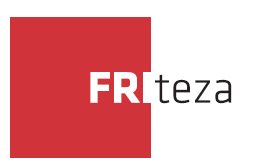
\includegraphics[width=\linewidth]{logo_fri.png}
\end{minipage}
\hfill
\begin{center}
{\Large \textbf{Coordinated UAV Swarm Target Defense Based on a Hawk–Pigeon Game}}\\[6pt]
{\large Micha Iakovlev, Hugo Trébert, Eliot Morin}\\[4pt]
Collective Behaviour Course, Research Seminar Report\\[4pt]
January 2026\\[10pt]
\textbf{Supervisor:} Iztok Lebar Bajec
\end{center}

\vspace{0.3cm}

\noindent

\vspace{0.3cm}
\hrule
\vspace{0.3cm}

\textbf{This paper presents a coordinated UAV swarm target defense strategy inspired by the Hawk–Pigeon Game. Building on analytical pursuit–evasion models introduced in previous work, we progressively refine the original framework to address practical limitations observed in multi-agent simulations. In particular, we introduce a hierarchical decision structure that separates global threat assessment from local pursuit control, combined with a predictive interception mechanism. Simulation results demonstrate that this approach improves interception efficiency, stability, and coordination compared to purely local or greedy strategies. While earlier reports envisioned learning-based extensions, this final work focuses on a robust deterministic baseline and discusses learning as future work.}

\vspace{0.3cm}
\hrule
\vspace{0.3cm}

% ====================
% MAIN TEXT
% ====================
\section{Introduction}

Unmanned aerial vehicle (UAV) swarms are increasingly employed in surveillance and defense applications, where they must operate under strict time constraints, limited sensing, and adversarial conditions. A representative scenario is target defense, in which a group of defender UAVs must intercept multiple attackers before they reach a protected asset. This problem is commonly modeled as a target–attacker–defender (TAD) pursuit–evasion game \cite{liang2019cooperative}.

Recent work has shown that bio-inspired approaches, particularly the Hawk–Pigeon Game, provide an effective analytical framework for swarm target defense \cite{ruan2021hawk}. In this model, defender UAVs (“hawks”) intercept attacking UAVs (“pigeons”) using biologically inspired targeting mechanisms and pursuit strategies. Analytical control laws such as proportional navigation (PN) and proportional pursuit (PP) offer interpretability and strong performance guarantees in simple scenarios \cite{zarchan2012missile}.

Our first reports implemented this framework and explored extensions toward imitation learning (IL) and reinforcement learning (RL). However, simulation analysis revealed that several structural limitations of the original Hawk–Pigeon formulation dominate performance before learning becomes relevant. In particular: purely local target selection leads to redundant pursuits, lack of anticipation causes inefficient tail-chasing, and absence of coordination prevents scalability.

In this final report, we present a polished and consolidated version of our previous work, focusing on a deterministic, interpretable solution that directly addresses these limitations. Learning-based approaches are deliberately postponed and discussed as future work. The source code used for all simulations and experiments presented in this paper
is publicly available at:
\url{https://github.com/eliotmorin18/uav-hawk-pigeon-swarm-defense}.

\section{Methods}

\subsection{Simulation Framework}

We consider a continuous-time two-dimensional UAV swarm defense scenario. Each unmanned aerial vehicle (UAV) is modeled as a second-order integrator:

\[
\dot{\mathbf{p}}_i = \mathbf{v}_i, \qquad 
\dot{\mathbf{v}}_i = \mathbf{u}_i,
\]

where $\mathbf{p}_i$ and $\mathbf{v}_i$ denote the position and velocity of UAV $i$, and $\mathbf{u}_i$ is the control input. The system dynamics are numerically integrated using a fourth-order Runge--Kutta scheme.

A fixed target must be defended from multiple attacking pigeons. Each hawk (defender UAV) is equipped with an omnidirectional sensor of radius $R_s$, meaning that only pigeons within this range are observable. A capture occurs when the distance between a hawk and a pigeon falls below a capture radius $D_c$. Hawks do not ``die'' during the simulation; failure corresponds to pigeons successfully reaching the protected target.

\subsection{Predictive Interception Control}

In the original Hawk--Pigeon model, hawks pursue the current position of their target, which frequently leads to tail-chasing behavior and overshoot \cite{brighton2019hawks}. To address this limitation, we introduce a predictive interception mechanism.

For each hawk--pigeon pair, the time-to-go $t_{go}$ is estimated under a constant-velocity assumption. The pigeon’s future position is predicted as:

\[
\mathbf{p}_{\text{pred}} = \mathbf{p} + \mathbf{v} \cdot t_{go}.
\]

To reduce sensitivity to noisy estimates, successive predictions are temporally blended. The resulting predicted position is then used as the reference for a combined proportional navigation (PN) and pure pursuit (PP) guidance law. This modification preserves analytical interpretability while significantly improving interception efficiency and trajectory smoothness.

\subsection{Global Threat Assessment}

A key limitation identified in earlier experiments was the purely local nature of target selection. To overcome this, we introduce a global threat (danger) evaluation computed at the game level.

For each pigeon, we estimate:
\begin{itemize}
    \item the time to reach the target $t_{\text{target}}$,
    \item the minimal achievable interception time $t_{\text{intercept}}$ across all hawks.
\end{itemize}

These quantities are combined into a continuous danger score that reflects both the urgency and the difficulty of interception. This reframes the defense problem from selecting the closest target to prioritizing the most threatening one.

\subsection{Coordinated Assignment and Stability}

Purely local decision-making in multi-agent systems is known to lead to redundant actions and inefficient resource usage, motivating explicit coordination mechanisms \cite{parker1998alliance}.

Using the ranked danger scores, hawks are explicitly assigned to pigeons through a one-to-one allocation procedure. Pigeons are processed in descending order of danger, and the best available hawk is assigned to each.

To prevent excessive target switching, an hysteresis mechanism is introduced: a hawk retains its current assignment unless a significantly more dangerous target appears. This stabilizes trajectories and reduces the erratic behavior observed in earlier versions of the model.

\paragraph{Author contributions.}
Eliot contributed to interception modeling and control refinement.
Hugo designed the global threat assessment and coordination architecture.
Micha performed simulation experiments and result analysis.

\section{Results}

All results presented in this section are obtained using the same initial
configuration with three defending hawks and five attacking pigeons.
Initial positions are fixed across all experiments to ensure a fair
comparison between methods. The only difference between configurations
lies in the enabled mechanisms: local decision-making, predictive
interception, and global coordination.

\subsection{Baseline Performance: Original Hawk--Pigeon Model}

We first evaluate the baseline Hawk--Pigeon model, in which each hawk
selects its target locally using proximity, margin, and density criteria
(T1/T2/T3), and pursues the instantaneous position of the selected pigeon
using a PN+PP guidance law.

Figure~\ref{fig:baseline_trajectories} shows the resulting 3D trajectories
for the considered 3v5 scenario. While hawks actively engage incoming
pigeons, the lack of coordination leads to frequent redundant pursuits,
with multiple hawks selecting the same target. As a consequence, some
pigeons remain unchallenged and are able to reach the protected target.

This behavior results in a mission failure: only three pigeons are
intercepted, while two successfully reach the target. The simulation
terminates after 7.68~s due to target capture (Table~\ref{tab:baseline_metrics}). These results highlight
the limitations of purely local decision-making in multi-defender
scenarios.

\begin{figure}[t]
    \centering
    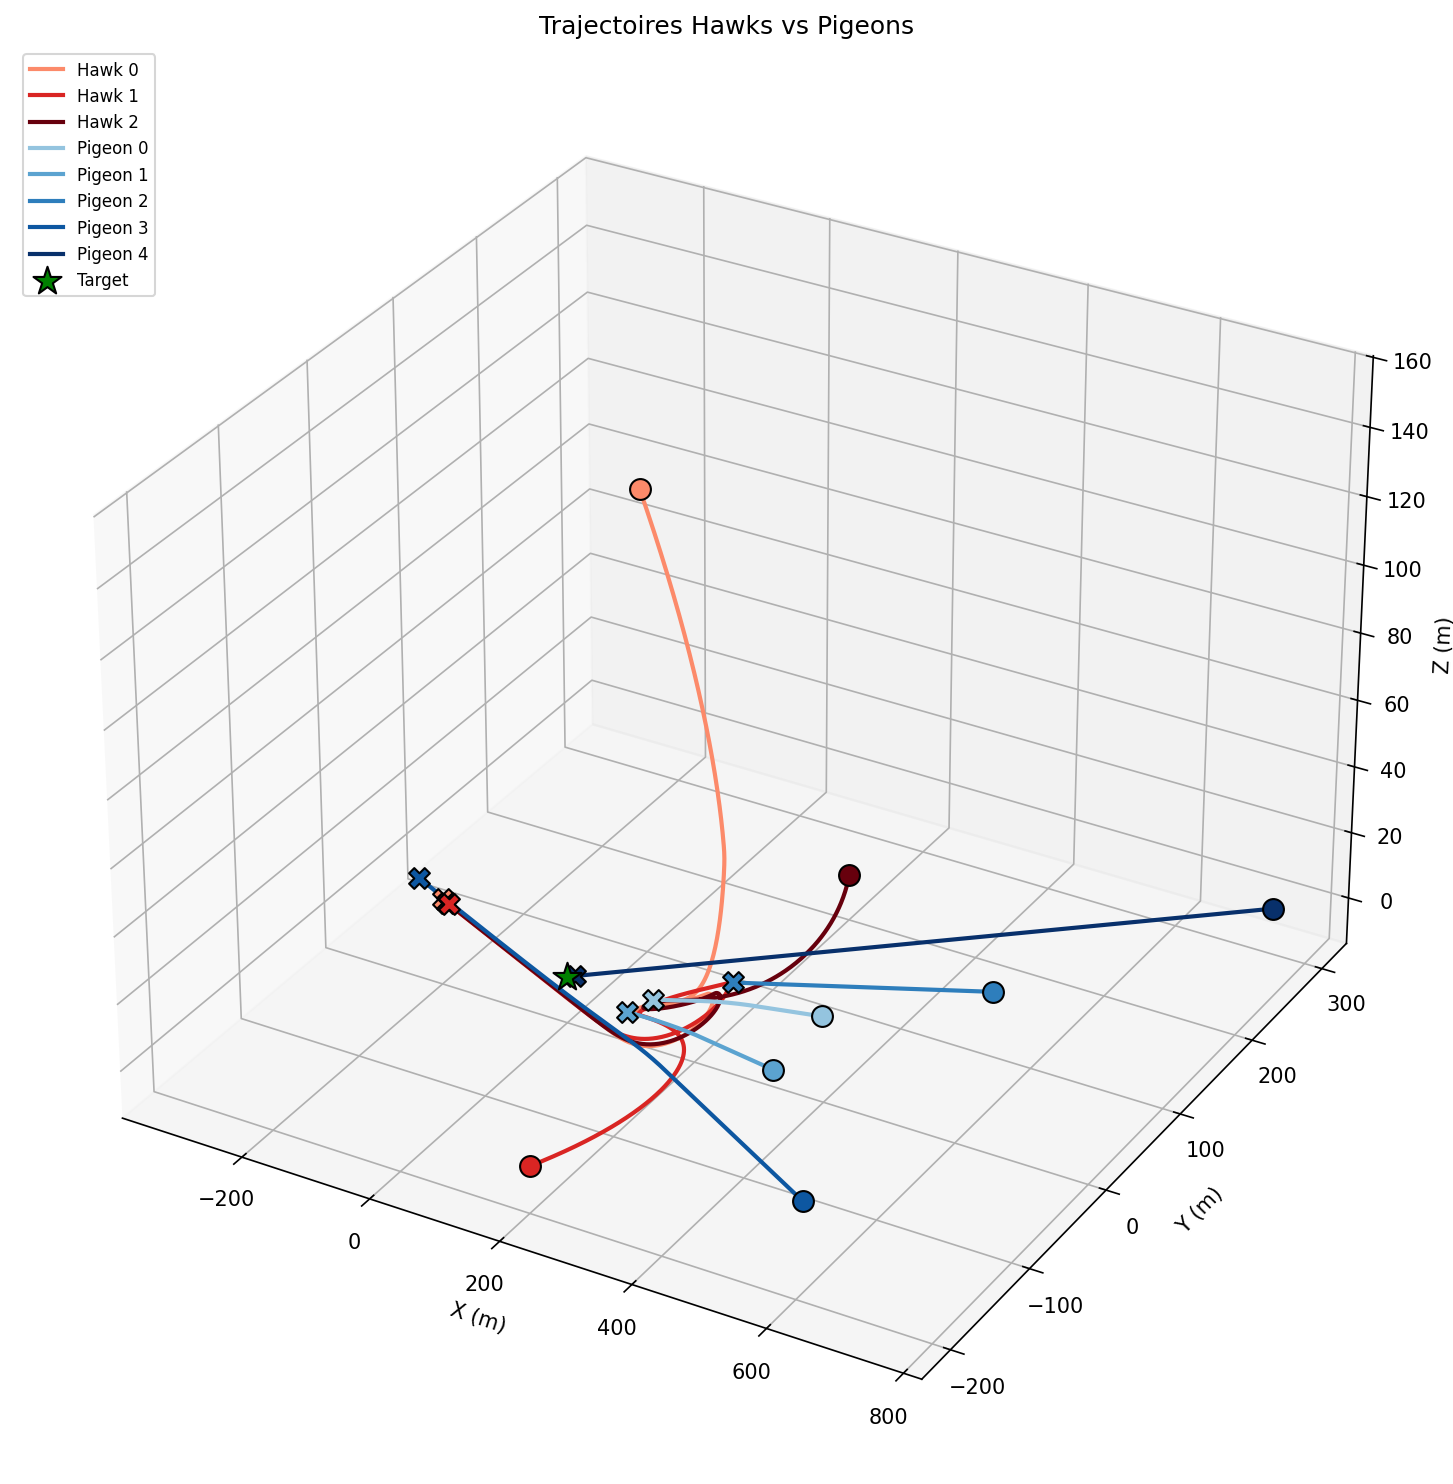
\includegraphics[width=0.9\linewidth]{plots/baseline_trajectories.png}
    \caption{3D trajectories of hawks and pigeons using the original
    Hawk--Pigeon model (paper mode). Redundant pursuits leave some
    pigeons unopposed.}
    \label{fig:baseline_trajectories}
\end{figure}

\begin{table}[t]
\centering
\caption{Outcome of the baseline Hawk--Pigeon model (3 hawks vs. 5 pigeons).}
\label{tab:baseline_metrics}
\resizebox{\columnwidth}{!}{%
\begin{tabular}{lc}
\hline
Metric & Value \\
\hline
Mission outcome & Target captured \\
Pigeons intercepted & 3 / 5 \\
Remaining pigeons & 2 \\
Simulation time (s) & 7.68 \\
\hline
\end{tabular}}
\end{table}

These results confirm that, although the original Hawk--Pigeon model
provides a sound analytical framework, its purely local target selection
strategy does not scale effectively when multiple defenders operate
simultaneously.

\subsection{Impact of Predictive Interception}

We next evaluate the effect of predictive interception while keeping the
original local target selection unchanged. 

Figure~\ref{fig:prediction_trajectories} illustrates the resulting
trajectories. Compared to the baseline case, hawk paths are more direct
and exhibit significantly reduced tail-chasing behavior. Interceptions
occur earlier, and the overall engagement is more stable.

In contrast to the baseline model, all five pigeons are successfully
intercepted before reaching the target. The total interception time is
reduced to 5.14~s (Table~\ref{tab:prediction_metrics}), demonstrating that anticipation alone substantially
improves interception efficiency, even in the absence of global
coordination.

\begin{figure}[t]
    \centering
    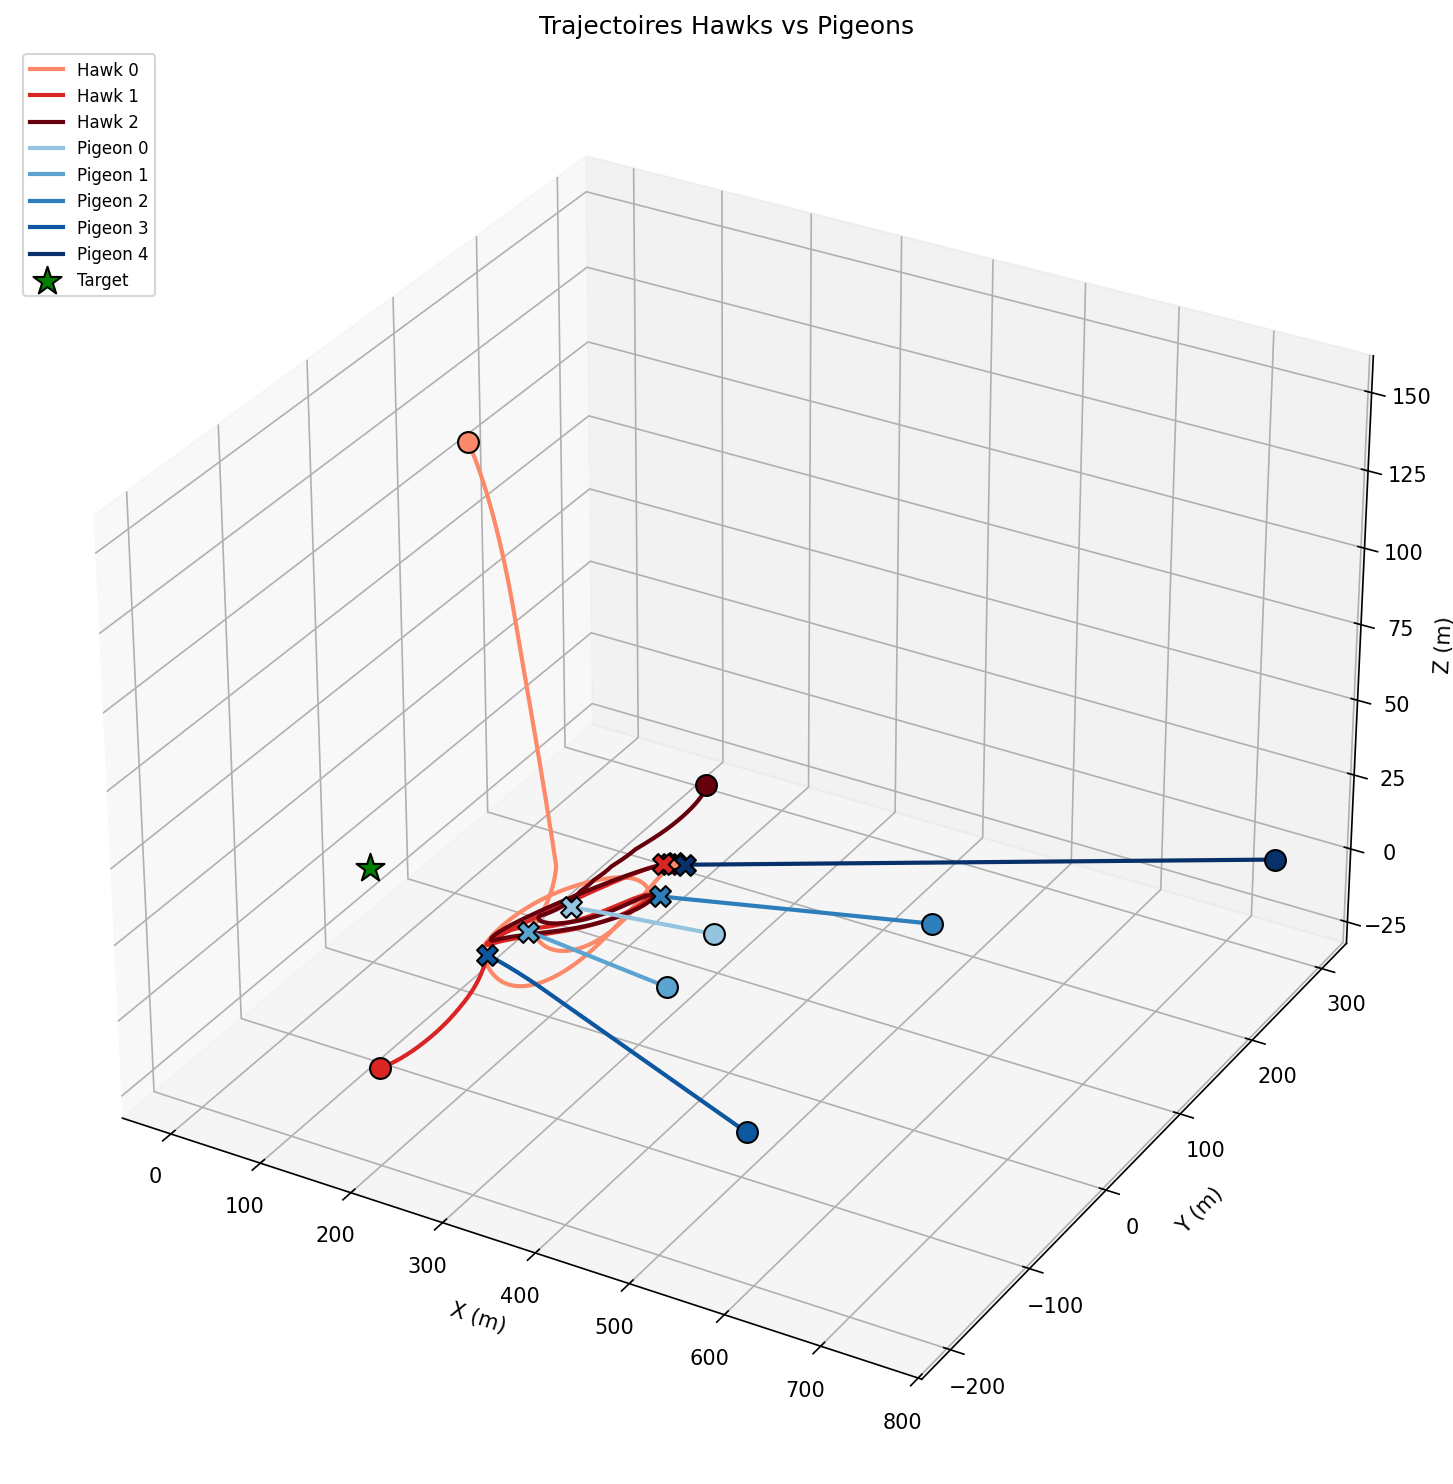
\includegraphics[width=0.9\linewidth]{plots/prediction_trajectories.png}
    \caption{3D trajectories using predictive interception with local
    target selection (paper\_anticipation mode).}
    \label{fig:prediction_trajectories}
\end{figure}

\begin{table}[t]
\centering
\caption{Effect of predictive interception without coordination (3v5).}
\label{tab:prediction_metrics}
\resizebox{\columnwidth}{!}{%
\begin{tabular}{lc}
\hline
Metric & Value \\
\hline
Mission outcome & All pigeons captured \\
Pigeons intercepted & 5 / 5 \\
Simulation time (s) & 5.14 \\
\hline
\end{tabular}}
\end{table}

These results show that predictive interception significantly enhances
individual pursuit performance, but does not address the underlying
coordination problem between multiple defenders.

\subsection{Effect of Danger-Based Global Coordination}

Finally, we evaluate the full proposed architecture, which combines
predictive interception with a global danger-based coordination mechanism.
In this configuration, pigeons are ranked according to a continuous danger
score based on their time to reach the target and the estimated
interception time. Hawks are then assigned to pigeons through a one-to-one
allocation process with hysteresis.

Figure~\ref{fig:coordination_trajectories} shows the resulting trajectories.
Hawks distribute themselves across the most threatening pigeons, avoiding
redundant pursuits and ensuring effective spatial coverage. No pigeon is
left unchallenged, and interceptions occur in a coordinated and orderly
manner.

All five pigeons are intercepted, and the total mission duration is
reduced to 3.69~s, representing a substantial improvement over both the
baseline and anticipation-only configurations.

\begin{figure}[t]
    \centering
    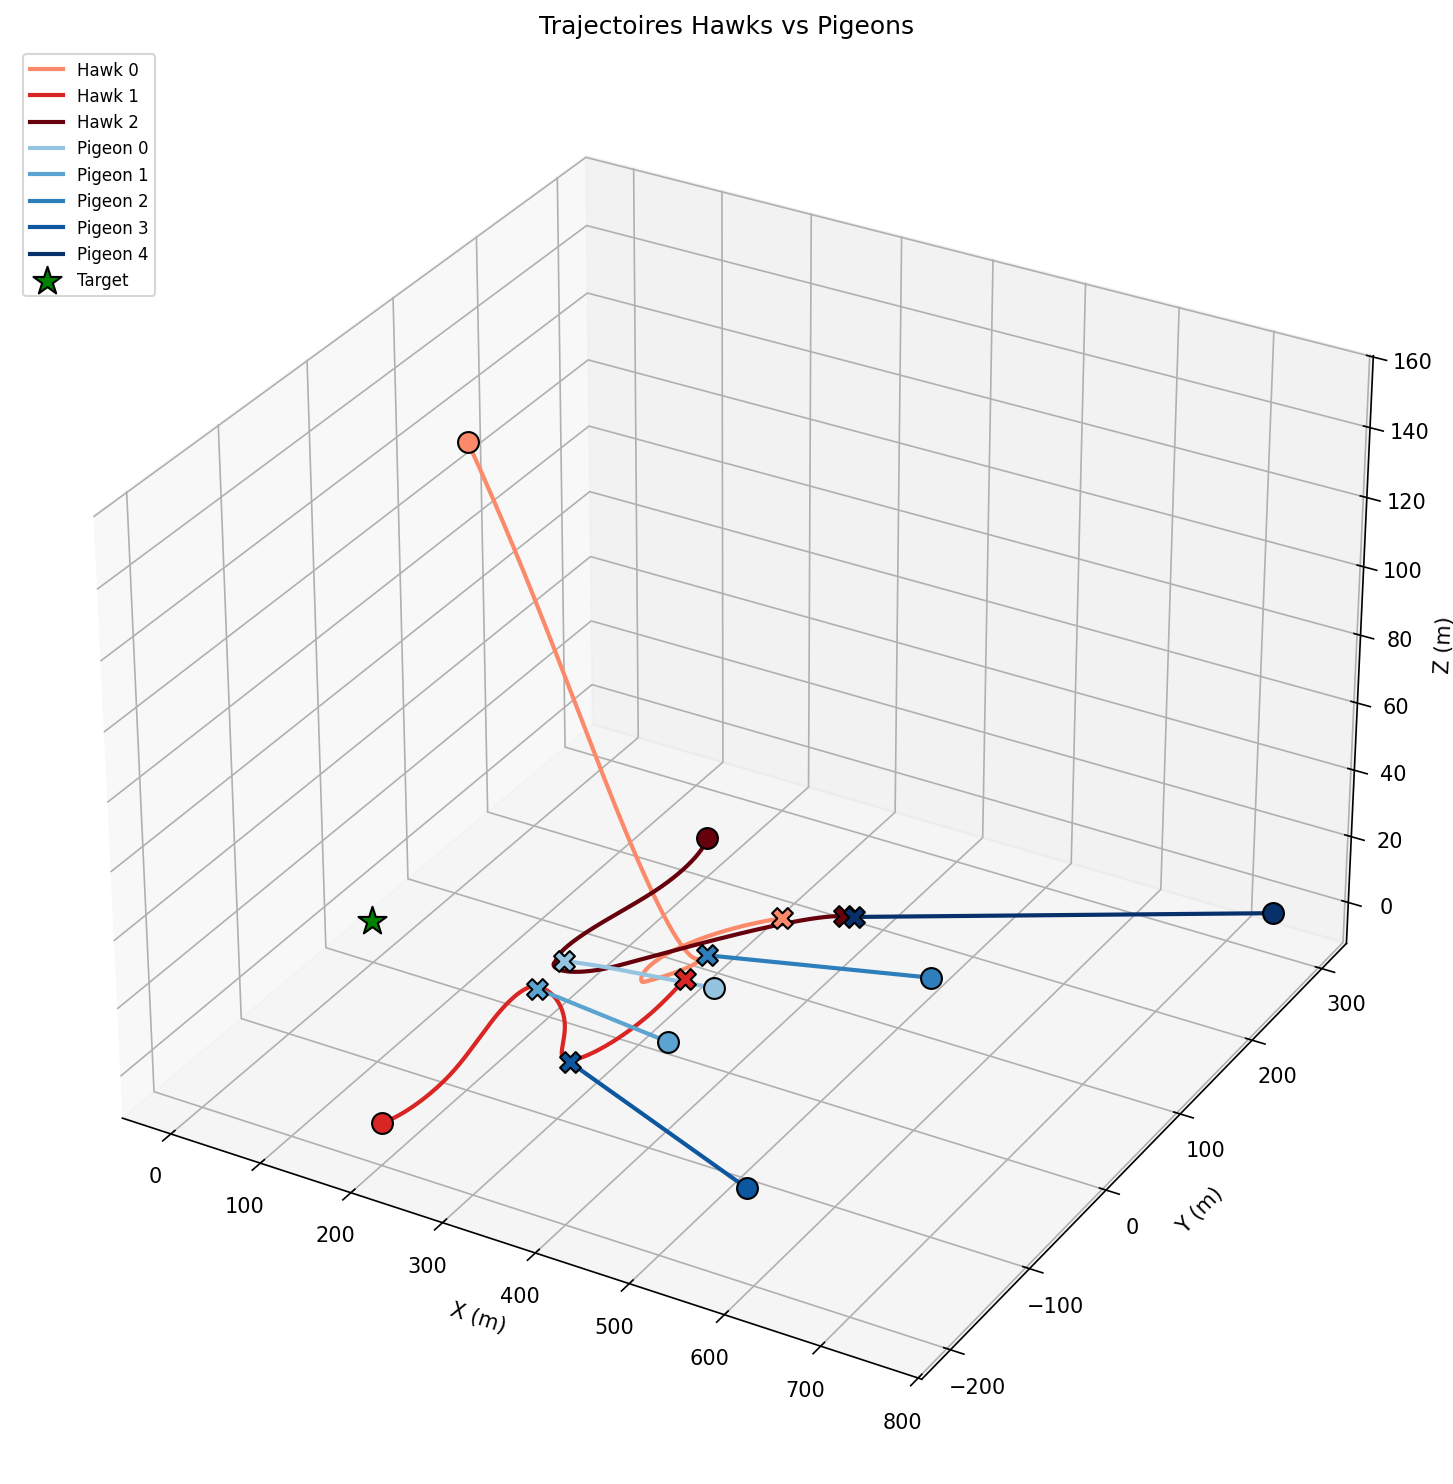
\includegraphics[width=0.9\linewidth]{plots/with_coordination.png}
    \caption{3D trajectories with danger-based global coordination (full
    mode).}
    \label{fig:coordination_trajectories}
\end{figure}

\begin{table}[t]
\centering
\caption{Comparison of the three configurations for the same 3v5 scenario.}
\label{tab:coordination_comparison}
\resizebox{\columnwidth}{!}{%
\begin{tabular}{lccc}
\hline
Metric & Paper & Paper + Anticipation & Full \\
\hline
Mission success & No & Yes & Yes \\
Pigeons intercepted & 3 / 5 & 5 / 5 & 5 / 5 \\
Simulation time (s) & 7.68 & 5.14 & 3.69 \\
\hline
\end{tabular}}
\end{table}

Overall, these results demonstrate that predictive interception improves
individual pursuit efficiency (Table~\ref{tab:coordination_comparison}), while danger-based global coordination is
essential to achieve robust and scalable target defense in multi-hawk
scenarios.





\section{Discussion}

Early versions of this project proposed extending the Hawk–Pigeon framework using imitation learning and reinforcement learning. However, experimental analysis revealed that unresolved coordination and stability issues would severely hinder learning performance. Addressing these issues deterministically proved both necessary and effective.

The architecture proposed here constitutes a strong analytical baseline that is interpretable, stable, and scalable. From this foundation, learning-based approaches could be meaningfully explored. For example, imitation learning could be used to approximate the coordinated control law, while reinforcement learning could refine local pursuit behaviors under uncertainty \cite{schulman2017ppo}.

Future work could also investigate decentralized implementations, more adversarial attacker behaviors, and extensions to three-dimensional dynamics.






\bibliographystyle{plain}
\bibliography{references}

\end{document}
